\documentclass[10pt,a4paper]{article}
\usepackage[margin=22mm]{geometry}
\usepackage[T1]{fontenc}
\usepackage{lmodern,amsmath,amssymb,booktabs,graphicx,tikz,hyperref,fvextra}
\usetikzlibrary{arrows.meta,positioning,calc,decorations.pathmorphing}
\definecolor{ink}{RGB}{20,53,78}
\hypersetup{colorlinks=true,urlcolor=ink,linkcolor=ink}
\setlength{\parindent}{0pt}
\setlength{\parskip}{5pt}
\emergencystretch=3em

\title{\color{ink}A passive notch filter and component tolerance}
\author{}
\date{Original learning collection -- November 2026}
\begin{document}
\begin{center}{\LARGE\color{ink}A passive notch filter and component tolerance}\\[5pt]{\small Original learning collection -- November 2026}\end{center}

\textbf{Evidence note.} Original teaching scenario. Numerical parameters are deliberately chosen for learning. All generated data and curves are synthetic; no physical measurement is asserted.
\section{Design brief}
An ideal voltage source drives series $R$, $L$ and $C$. Measure the combined voltage $y=v_L+v_C$. Use $L=10\,\mathrm{mH}$, $C=100\,\mu\mathrm{F}$ and $R=10\,\Omega$. Derive the notch transfer, compare it with the capacitor-voltage response, and evaluate the effect of a $\pm10\%$ capacitance tolerance. Assume ideal components and an unloaded measurement.
\section{Physical system}
\begin{center}\resizebox{\ifdim\width>.98\linewidth.98\linewidth\else\width\fi}{!}{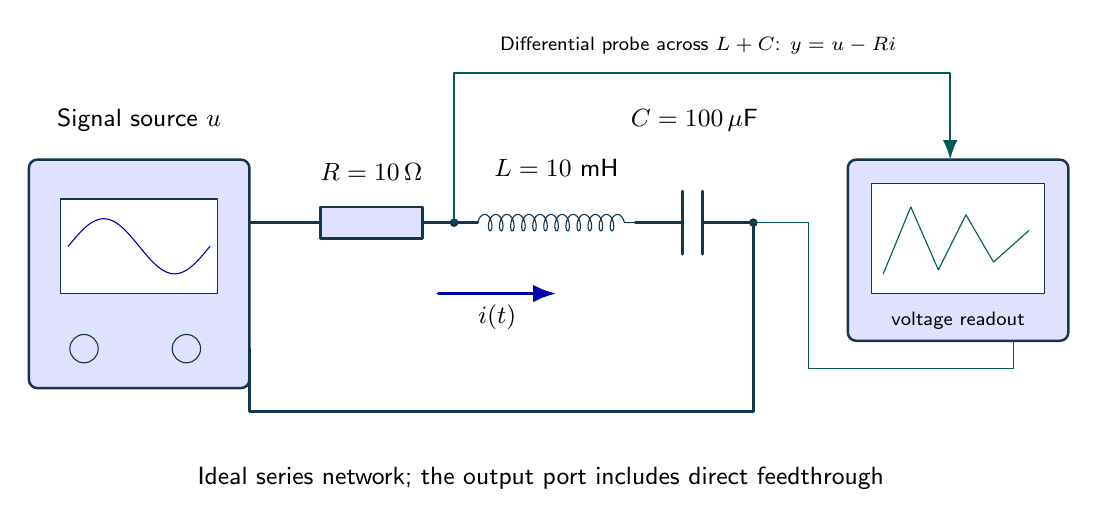
\begin{tikzpicture}[
font=\sffamily\small,>=Latex,line cap=round,line join=round,
wall/.style={draw=ink,line width=1.2pt,fill=blue!5},
water/.style={fill=cyan!25,draw=none},
metal/.style={draw=ink,fill=blue!12,line width=.9pt},
flow/.style={->,draw=blue!65!black,line width=1.2pt},
heat/.style={->,draw=orange!85!black,line width=1.1pt},
measure/.style={->,draw=teal!70!black,line width=.9pt},
dim/.style={<->,draw=ink!65,line width=.6pt},
spring/.style={draw=ink,decorate,decoration={coil,aspect=.5,segment length=4pt,amplitude=3pt}},
wire/.style={draw=ink,line width=1pt},
lab/.style={align=center,font=\sffamily\small},
smalllab/.style={align=center,font=\sffamily\scriptsize}]

\draw[metal,rounded corners=3pt](.3,1.1)rectangle(3.1,4);
\draw[fill=white,draw=ink](.7,2.3)rectangle(2.7,3.5);
\draw[blue!70!black,domain=.8:2.6,samples=60]plot(\x,{2.9+.35*sin(360*(\x-.8)/1.8)});
\draw[ink](1,1.6)circle(.18)(2.3,1.6)circle(.18);
\node[lab]at(1.7,4.5){Signal source $u$};
\draw[wire](3.1,3.2)--(4,3.2);
\draw[metal](4,3)rectangle(5.3,3.4);
\node[lab]at(4.65,3.85){$R=10\,\Omega$};
\draw[wire](5.3,3.2)--(6,3.2);
\draw[spring](6,3.2)--(8,3.2);
\draw[wire](8,3.2)--(8.6,3.2);
\draw[wire](8.6,2.8)--(8.6,3.6)(8.85,2.8)--(8.85,3.6);
\draw[wire](8.85,3.2)--(9.5,3.2)--(9.5,.8)--(3.1,.8)--(3.1,1.6);
\node[lab]at(7,3.9){$L=10$ mH};
\node[lab]at(8.75,4.5){$C=100\,\mu$F};
\draw[flow](5.5,2.3)--(7,2.3)node[midway,below]{$i(t)$};
\draw[metal,rounded corners=3pt](10.7,1.7)rectangle(13.5,4);
\draw[fill=white,draw=ink](11,2.3)rectangle(13.2,3.7);
\draw[teal!70!black](11.15,2.55)--(11.5,3.4)--(11.85,2.6)--(12.2,3.3)--(12.55,2.7)--(13,3.1);
\node[smalllab]at(12.1,1.95){voltage readout};
\fill[ink](5.7,3.2)circle(.055)(9.5,3.2)circle(.055);
\draw[measure](5.7,3.2)--(5.7,5.1)--(12,5.1)--(12,4);
\draw[teal!70!black](9.5,3.2)--(10.2,3.2)--(10.2,1.35)--(12.8,1.35)--(12.8,1.7);
\node[smalllab]at(8.8,5.45){Differential probe across $L+C$: $y=u-Ri$};
\node[lab]at(6.8,-.05){Ideal series network; the output port includes direct feedthrough};
\end{tikzpicture}
}\par{\small A source excites the series RLC network; an ideal differential probe spans the combined inductor and capacitor. Measuring only the capacitor would produce a different transfer function. Wire placement is schematic.}\end{center}
\section{Voltage division}
The impedances are $Z_R=R$, $Z_L=sL$ and $Z_C=1/(sC)$. Measuring across the combined LC section gives
\[G_n(s)=\frac{sL+1/(sC)}{R+sL+1/(sC)}=\frac{LCs^2+1}{LCs^2+RCs+1}.\]
Measuring across C alone instead gives $G_C(s)=1/(LCs^2+RCs+1)$. Both share poles, but their zeros and frequency responses differ.
\section{Nominal design}
Here $LC=10^{-6}$ s$^2$, $RC=10^{-3}$ s, $\omega_0=1/\sqrt{LC}=1000$ rad/s and $\zeta=(R/2)\sqrt{C/L}=0.5$. The notch has zeros at $\pm j1000$ and stable poles $-500\pm j866.0254$. Its DC and high-frequency gains are one.
\section{Tolerance analysis}
At ideal resonance, the inductor and capacitor voltages cancel in their sum. A capacitance factor $a$ moves the notch to $\omega_0/\sqrt a$; a 10 percent tolerance is not a symmetric 10 percent frequency change. The first-order sensitivity is $\delta\omega_0/\omega_0\simeq-\delta C/(2C)$.
\section{Physical interpretation}
A zero in the measured sum does not mean zero branch current or zero energy in the individual elements. Resistance in the inductor, source impedance and output loading reduce notch depth and alter the ideal transfer function. The logarithmic plot is clipped only for display at very small magnitudes.
\section{What to learn from the experiment}
Output selection changes zeros even when the physical circuit is unchanged. An ideal notch is sensitive to component tolerance and omitted losses.
\section{System sketch}
\begin{center}\resizebox{\ifdim\width>.98\linewidth.98\linewidth\else\width\fi}{!}{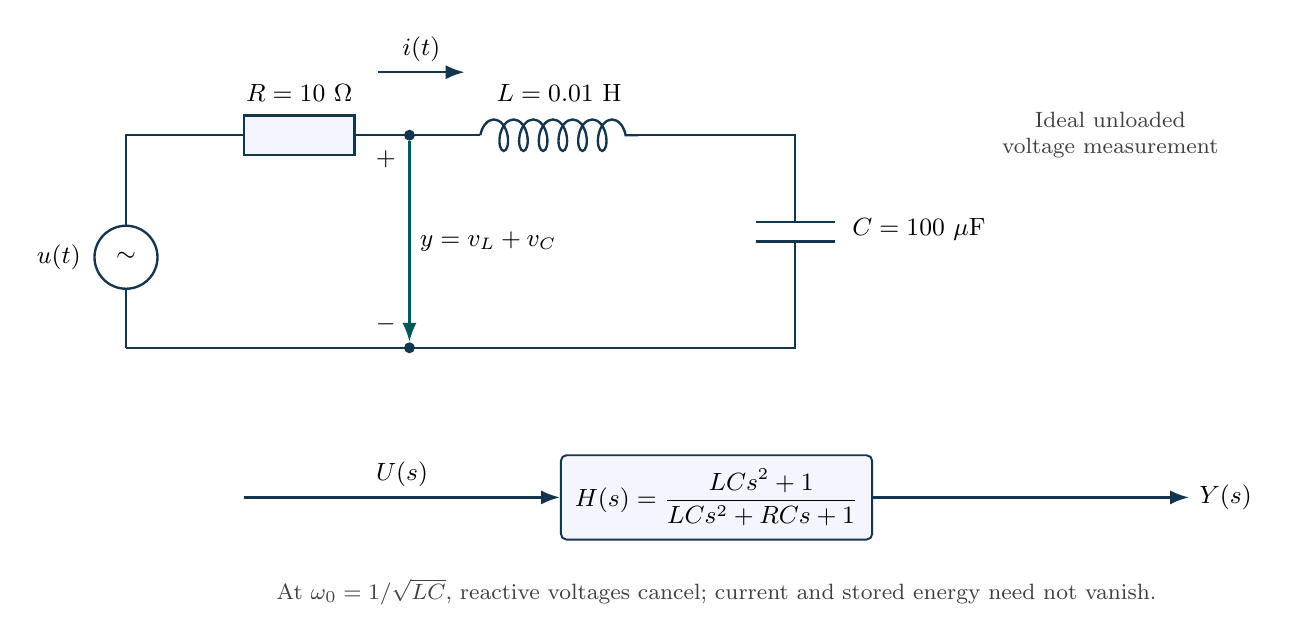
\begin{tikzpicture}[x=1cm,y=1cm,>=Latex,font=\small,
block/.style={draw=ink,fill=blue!4,rounded corners=2pt,minimum height=9mm,align=center,line width=.7pt,inner sep=5pt},
sum/.style={circle,draw=ink,fill=white,minimum size=6mm,inner sep=0pt,line width=.7pt},
sig/.style={->,draw=ink,line width=.85pt},
fb/.style={->,draw=teal!70!black,line width=.85pt},
dist/.style={->,draw=orange!75!black,line width=.85pt},
tap/.style={circle,fill=ink,inner sep=1.4pt},
note/.style={font=\footnotesize,align=center,text=black!75}]

\draw[draw=ink,line width=.85pt](.5,.3)--(.5,1.05);
\draw[draw=ink,line width=.85pt](.5,1.45)circle(.4);
\node at(.5,1.45){$\sim$};
\draw[draw=ink,line width=.85pt](.5,1.85)--(.5,3)--(2,3);
\node[left]at(.05,1.45){$u(t)$};
\draw[draw=ink,fill=blue!4,line width=.85pt](2,2.75)rectangle(3.4,3.25);
\node[above]at(2.7,3.3){$R=10\ \Omega$};
\draw[draw=ink,line width=.85pt](3.4,3)--(5,3);
\draw[decorate,decoration={coil,aspect=.55,segment length=2.5mm,amplitude=2mm},line width=.85pt,draw=ink](5,3)--(7,3);
\node[above]at(6,3.3){$L=0.01\ \mathrm{H}$};
\draw[draw=ink,line width=.85pt](7,3)--(9,3)--(9,1.9);
\draw[line width=.85pt,draw=ink](8.5,1.9)--(9.5,1.9)(8.5,1.65)--(9.5,1.65);
\draw[line width=.85pt,draw=ink](9,1.65)--(9,.3)--(.5,.3);
\node[right]at(9.6,1.8){$C=100\ \mu\mathrm{F}$};
\draw[sig](3.7,3.8)--node[above]{$i(t)$}(4.8,3.8);
\node[tap](a)at(4.1,3){};\node[tap](b)at(4.1,.3){};
\draw[fb](a)--node[right]{$y=v_L+v_C$}(b);
\node at(3.8,2.7){$+$};\node at(3.8,.6){$-$};
\node[note]at(13,3){Ideal unloaded\\voltage measurement};
\node[block](h)at(8,-1.6){$H(s)=\dfrac{LCs^2+1}{LCs^2+RCs+1}$};
\draw[sig](2,-1.6)--node[above]{$U(s)$}(h);
\draw[sig](h)--(14,-1.6)node[right]{$Y(s)$};
\node[note]at(8,-2.8){At $\omega_0=1/\sqrt{LC}$, reactive voltages cancel; current and stored energy need not vanish.};

\end{tikzpicture}
}
\par\small\refstepcounter{figure}\label{fig:system}\textbf{Figure \thefigure.} Series RLC network with output measured across L and C together. The output probe spans those two components, not the whole source.\end{center}
\section{Executed computational evidence}
\VerbatimInput[fontsize=\small,breaklines=true]{results.txt}
\begin{center}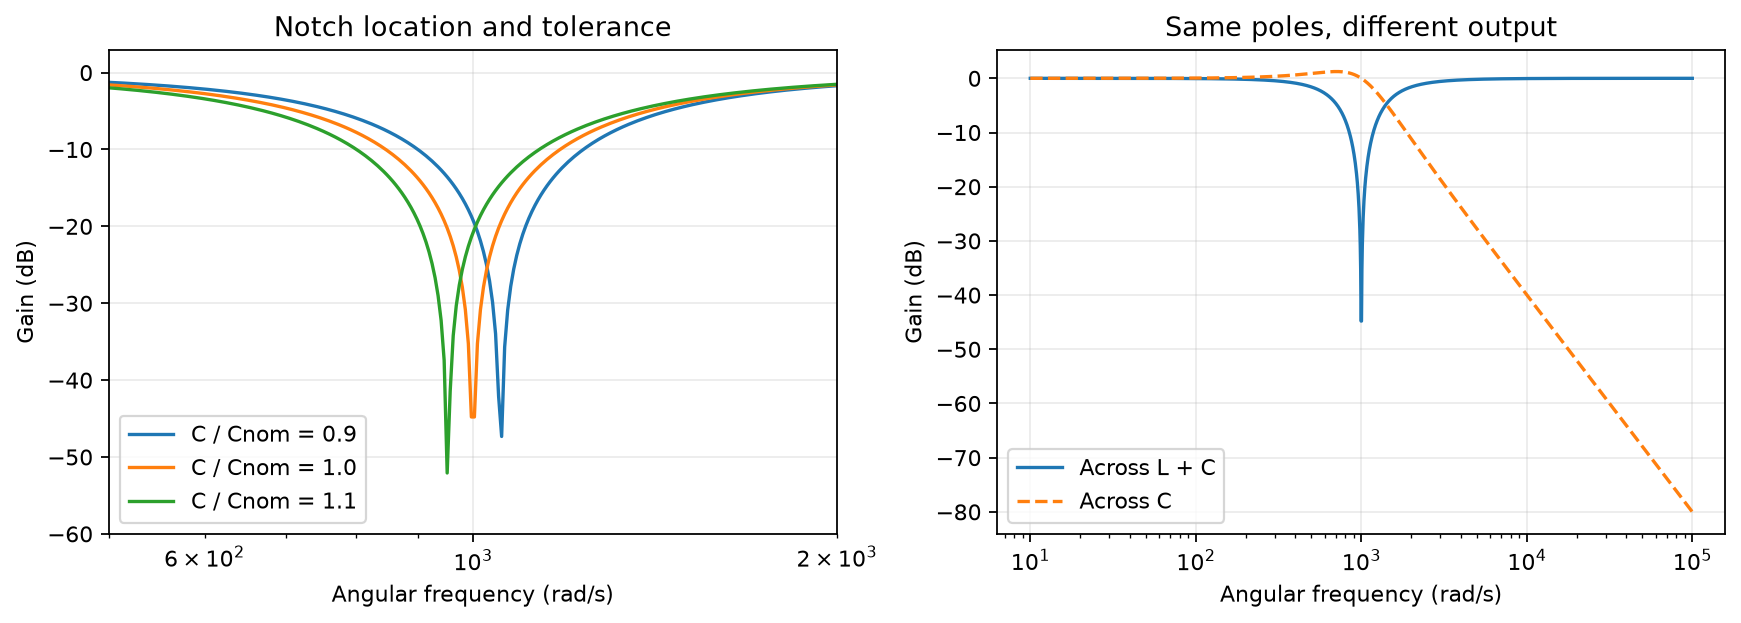
\includegraphics[width=\linewidth,height=.16\textheight,keepaspectratio]{response.png}\end{center}
\paragraph{Method references.}
The equations use standard balance laws and feedback-control methods. Further explanation: \url{https://apmonitor.com/pdc/} and \url{https://fbsbook.org/}. Implementation documentation: \url{https://python-control.readthedocs.io/en/0.10.2/}. See the repository reference catalog for individual topics and videos.
\end{document}
